\documentclass{article}
\usepackage[margin=2cm]{geometry}
\usepackage{graphicx}
\usepackage[pages=some]{background}
\usepackage{titling}
\usepackage{tabularx}
\usepackage{multicol}
\usepackage{amsmath}
\usepackage{amssymb}
\usepackage{subfigure}
% \usepackage{tikz}
% \usepackage{fontspec}

% \newfontfamily\bengalifont{Kalpurush}[Script=Bengali,Scale=0.9]

\backgroundsetup{
    scale=1,
    angle=0,
    opacity=1,
    contents={%
        
\includegraphics[width=\paperwidth,height=\paperheight]{institution_logo.jpg}
    }
}

\newcommand{\subtitle}[1]{
    \posttitle{
        \par\end{center}
        \begin{center}\large#1\end{center}
        \vskip0.5em}
}

\title{ME-463}
\author{Md. Hasibul Islam}
\subtitle{PETROLEUM ENGINEERING}

\begin{document}
\begin{titlepage}
    \centering
    
    {\Huge\bfseries\maketitle}
    \textbf{Nasim Hasan Sir} \\
    \vspace{2cm}
    
\includegraphics[width=8cm]{institution_logo.jpg}
    \vfill
\end{titlepage}

\tableofcontents
\pagebreak

\section{Lecture 01: Introduction} 
\hfill Date: 04/06/2023
\subsubsection*{[See The Other PDF/Tex file]}

\section{Lecture 2: Petroleum Overviews \& Formations} 
\hfill Date: 06/06/2023

\subsubsection*{Petroleum}
Petroleum is a naturally occurring, flammable liquid that is found beneath the Earth's surface. It is a complex mixture of hydrocarbons, which are organic compounds consisting primarily of carbon and hydrogen atoms. Petroleum is commonly referred to as crude oil and serves as a vital source of energy worldwide. It is refined to produce various fuels such as gasoline, diesel, and jet fuel, as well as other products like lubricants, plastics, and chemicals. The exploration, extraction, refining, and distribution of petroleum are integral to the petroleum industry, which plays a significant role in the global economy.\\
Petroleum is natural accumulation of organic matters. It may be gaseous, liquid or semi-solid substance. 

\subsubsection*{Different stages}
Diagenesis, catagenesis, and metagenesis are terms used to describe different stages of organic matter transformation within the Earth's subsurface. These processes occur over long periods of time and under specific temperature, pressure, and geological conditions. Here are their characteristics:

\textbf{Diagenesis}:
    \begin{itemize}
        \item Diagenesis is the earliest stage of organic matter transformation.
        \item It occurs at relatively low temperatures and pressures.
        \item Organic matter undergoes physical and chemical changes, such as compaction, dissolution, and microbial degradation.
        \item Diagenesis typically happens within the upper few kilometers of the Earth's crust.
        \item The primary result of diagenesis is the formation of sedimentary rocks.
    \end{itemize}


\textbf{Catagenesis}:
    \begin{itemize}
        \item Catagenesis is the intermediate stage between diagenesis and metagenesis.
        \item It occurs at higher temperatures and pressures than diagenesis, typically within the range of 60 to 150 degrees Celsius.
        \item Organic matter undergoes thermal decomposition, leading to the formation of hydrocarbons.
        \item The process of catagenesis is responsible for the generation of petroleum and natural gas.
        \item It is commonly associated with the burial of organic-rich sediments and the subsequent heating over geologic time.
    \end{itemize}

\textbf{Metagenesis}:
    \begin{itemize}
        \item Metagenesis is the final stage of organic matter transformation.
        \item It occurs at higher temperatures and pressures than catagenesis, typically above 150 degrees Celsius.
        \item Organic matter is subjected to extensive thermal cracking, resulting in the production of graphite, carbon dioxide, and other inorganic compounds.
        \item Metagenesis is associated with deep burial and metamorphism of organic-rich rocks.
        \item The process of metagenesis is responsible for the formation of metamorphic rocks.
    \end{itemize}


\subsubsection*{Kerogen}
Kerogen refers to the organic matter found in sedimentary rocks that has the potential to generate hydrocarbons through processes like catagenesis. Kerogen is classified into different types based on its composition and characteristics. The four types of kerogen are Type I, Type II, Type III, and Type IV. Here are their characteristics:\\

\textbf{Type I Kerogen}:
    \begin{itemize}
        \item Type I kerogen is derived from organic material rich in hydrogen and relatively low in oxygen.
        \item It has a high hydrogen-to-carbon (H/C) ratio and a high potential for oil generation.
        \item Type I kerogen is typically found in organic-rich marine environments, such as shale formations associated with ancient lakes or marine basins.
        \item It generates primarily liquid hydrocarbons, including oil and gas.
    \end{itemize}

\textbf{Type II Kerogen}:
    \begin{itemize}
        \item Type II kerogen is derived from a mixture of marine and terrestrial organic matter.
        \item It has a moderate hydrogen-to-carbon (H/C) ratio.
        \item Type II kerogen is commonly found in shale formations and coal deposits.
        \item It has a moderate potential for hydrocarbon generation and can generate both oil and gas.
    \end{itemize}

\textbf{Type III Kerogen}:
    \begin{itemize}
        \item Type III kerogen is derived from terrestrial organic matter, such as woody plant material and lignite coal.
        \item It has a relatively low hydrogen-to-carbon (H/C) ratio and a high oxygen content.
        \item Type III kerogen is typically found in coal deposits and can generate mainly gas during thermal maturation.
    \end{itemize}

\textbf{Type IV Kerogen}:
    \begin{itemize}
        \item Type IV kerogen consists of highly mature and degraded organic matter.
        \item It has a low hydrogen-to-carbon (H/C) ratio and a high carbon content.
        \item Type IV kerogen is commonly found in highly metamorphosed rocks, such as graphite-rich metamorphic rocks.
        \item It has a very low potential for hydrocarbon generation.
    \end{itemize}

\subsubsection*{Maturation of Kerogen}
The maturity of kerogen refers to the level of thermal alteration and maturation it has undergone. It is an important parameter in understanding the potential for hydrocarbon generation from organic-rich rocks. Here are some key aspects related to the maturity of kerogen:\\

\textbf{Maturity Parameters}:
    \begin{itemize}
        \item \textbf{Vitrinite Reflectance (\%Ro)}: Vitrinite reflectance is a widely used parameter to assess the thermal maturity of kerogen. It measures the reflectance of vitrinite macerals under a microscope and increases with increasing thermal maturity. The \%Ro value is commonly used as a quantitative indicator of kerogen maturity.
        \item \textbf{Tmax}: Tmax is the temperature at which the maximum rate of hydrocarbon generation occurs during the thermal maturation of kerogen. It is often used as an indicator of thermal maturity and can be determined through laboratory pyrolysis experiments.
        \item \textbf{SCI (S1 Peak Height)}: Obtained from Rock-Eval pyrolysis, it measures the amount of hydrocarbons generated during pyrolysis. As kerogen matures, the S1 peak height increases, indicating higher thermal breakdown and hydrocarbon generation. SCI is expressed as the ratio of S1 peak height to total organic carbon (TOC) content.
        \item \textbf{TAI (Thermal Alteration Index)}: TAI qualitatively assesses thermal maturity based on visual examination. It involves observing changes in kerogen's color, reflectance, and isotropy under a microscope. TAI ranges from TAI-1 (low maturity) to TAI-4 (high maturity), indicating increasing thermal alteration.
    \end{itemize}

\textbf{Maturation Indicators}:
    \begin{itemize}
        \item \textbf{Hydrocarbon Generation}: As kerogen matures, it undergoes thermal decomposition and generates hydrocarbons. The type and amount of hydrocarbons generated are indicative of the maturation level.
        \item \textbf{Changes in Organic Petrography}: The microscopic examination of organic matter can reveal changes in its structure, such as the disappearance of certain organic components or the alteration of reflectance values, which indicate the maturation stage.
        \item \textbf{Thermal Alteration of Biomarkers}: Biomarkers are organic compounds derived from specific organisms and can be preserved in sedimentary rocks. As kerogen matures, biomarkers undergo thermal alteration, such as changes in their structure or ratios, which can be used as indicators of maturation.
    \end{itemize}



\textbf{Maturation Factors}:
    \begin{itemize}
        \item \textbf{Temperature}: Higher temperatures accelerate the maturation process of kerogen. The geothermal gradient, burial depth, and tectonic activity in a particular area influence the temperature conditions experienced by kerogen.
        \item \textbf{Time}: Maturation is a time-dependent process. The longer the organic-rich rocks are subjected to elevated temperatures, the more advanced the maturation becomes.
        Organic Matter Type: The type of organic matter (e.g., marine, terrestrial) and its composition (e.g., hydrogen-to-carbon ratio, oxygen content) influence the maturation characteristics and the types of hydrocarbons generated.
        \item \textbf{Thermal Conductivity of Surrounding Rocks}: The thermal conductivity of the rocks surrounding the organic-rich source rocks affects the rate at which heat is conducted, influencing the maturation process.
    \end{itemize}

    \subsubsection*{Wet Gas}
    Wet gas is a natural gas mixture that contains significant amounts of natural gas liquids (NGLs) along with methane. It has a higher energy content and requires additional processing to separate and recover the NGLs. The extracted NGLs have various applications, such as petrochemical feedstocks and fuels. Wet gas reserves are economically valuable due to the additional revenue from NGLs. Understanding wet gas is essential for effective exploration, production, and processing of natural gas resources.\\ 


    \section{Lecture 3: Petroleum Overviews \& Formations}
    \hfill Date: 14/06/2023
    
    [see slide no. 2 of Nasim Sir]

    \section{Lecture 4: Reservoir Rocks \& Their Properties}
    \hfill Date: 20/06/2023

    \subsection*{Reservoir Rocks} 
    Reservoir rocks are the types of rocks that contain and hold significant amounts of oil, gas, or water that can be economically extracted. These rocks have the capability to store and transmit fluids such as hydrocarbons (oil and gas) or water. Reservoir rocks are typically porous and permeable, allowing the movement of fluids through interconnected pore spaces.

The main types of reservoir rocks include:
\begin{enumerate}
    \item \textbf{Sandstone}: Sandstone reservoir rocks are composed of consolidated grains of sand. They are commonly found in sedimentary basins and often have good porosity and permeability properties, making them excellent reservoirs for oil and gas.
    \item \textbf{Carbonate}: Carbonate reservoir rocks are composed primarily of calcium carbonate minerals, such as limestone and dolomite. They are formed in marine environments and can have complex pore systems, including vugs and fractures, which can significantly impact their reservoir properties.
    \item \textbf{Shale}: Shale reservoir rocks are fine-grained sedimentary rocks composed of clay minerals and organic matter. While shale itself is not typically a good reservoir rock due to its low permeability, it can act as a source rock, generating and supplying hydrocarbons to adjacent reservoir rocks.
    \item \textbf{Clays}: Clays are fine-grained sedimentary rocks composed primarily of clay minerals. While clays themselves have low permeability, they can play a significant role in reservoir systems. Clay minerals can act as cap rocks, sealing the reservoir and preventing the migration of fluids. They can also influence the reservoir's mechanical properties and fluid behavior due to their swelling or compaction characteristics.
    \item \textbf{Igneous and Metamorphic Rocks}: While sedimentary rocks are the most common types of reservoir rocks, certain igneous and metamorphic rocks can also serve as reservoirs. Igneous rocks, such as volcanic rocks or intrusive igneous formations, can have interconnected fractures or vesicles that can store and transmit fluids. Metamorphic rocks, which have undergone intense heat and pressure, can develop secondary porosity and permeability through processes like fracturing and dissolution.
    \item \textbf{Limestone}: Limestone reservoir rocks are primarily composed of calcium carbonate. They can have varying degrees of porosity and permeability, depending on factors such as the presence of fractures and the degree of diagenetic alteration.
    \item Siltstone: Siltstone reservoir rocks are fine-grained sedimentary rocks composed of silt-sized particles. They have moderate porosity and permeability and can serve as reservoirs for oil, gas, or water in certain geological settings.
\end{enumerate}


\subsection*{Other Properties}
\begin{itemize}
    \item Fluid Saturation: Fluid saturation refers to the amount of pore space occupied by fluids (e.g., oil, gas, water) within a reservoir rock. It is expressed as a fraction or percentage and is important for estimating the amount of recoverable hydrocarbons in a reservoir.
    \item Wettability: Wettability describes the affinity of a reservoir rock's surface for a particular fluid phase (e.g., oil, water). It influences the distribution and movement of fluids within the rock and affects the efficiency of oil recovery processes.
    \item Surface and Interfacial Tension: Surface tension is the property of a fluid that causes its surface to behave like a stretched elastic membrane. Interfacial tension refers to the tension between two immiscible fluids at their interface. These tensions play a role in capillary forces and can affect fluid flow and displacement in porous media.
    \item Capillary Pressure: Capillary pressure is the pressure difference across the interface of two immiscible fluids within a porous medium. It is caused by the capillary forces within the small pores of the rock and influences fluid movement and saturation distribution.
    \item Rock Compressibility: Rock compressibility measures the change in rock volume or porosity in response to changes in pressure. It is an important factor in reservoir engineering calculations, such as estimating reservoir volume changes during production.
    \item Overburden Pressure: Overburden pressure, also known as lithostatic pressure, is the vertical pressure exerted on a reservoir rock by the weight of the overlying rock layers. It increases with depth and affects the effective stress within the rock, influencing its mechanical and fluid flow properties.
\end{itemize}


\subsection*{Porosity}
Porosity refers to the percentage of void space (pore volume) within a rock or sediment. In the context of reservoir rocks, porosity is a crucial property that determines the rock's ability to store and transmit fluids such as oil, gas, or water.\\

Reservoir rocks with high porosity have a greater volume of interconnected pore spaces, providing more room for fluid storage. Conversely, rocks with low porosity have fewer pore spaces and therefore less capacity to hold fluids. Porosity is typically expressed as a fraction or percentage.\\

Porosity is a fundamental parameter in reservoir characterization and evaluation. It is used to estimate the total volume of hydrocarbons that a reservoir can potentially hold. Combined with other factors like fluid saturation, it helps determine the total volume of recoverable hydrocarbons.\\

Different rock types have varying inherent porosity. For example, sandstones often exhibit higher porosity due to their relatively large and interconnected pore spaces, while shale or carbonate rocks tend to have lower porosity due to their more compact and less interconnected pore structure.\\ 

\textbf{ Porosity is the capability of a rock to hold fluids in pore.
It is the ratio of the pore volume in a rock to the bulk volume of that
rock. Expressed in per cent.}\\

The mathematical expression:
$$\Phi = \frac{V_p}{V_b}$$

Where, $V_P$ is the total volume of pore space and $V_b$ is the total volume of rock or sediment.\\

\textbullet Porosity varies from 0\% to 70\% in natural sediments and exceeds 70\% for freshly deposited mud.  

\begin{figure}
    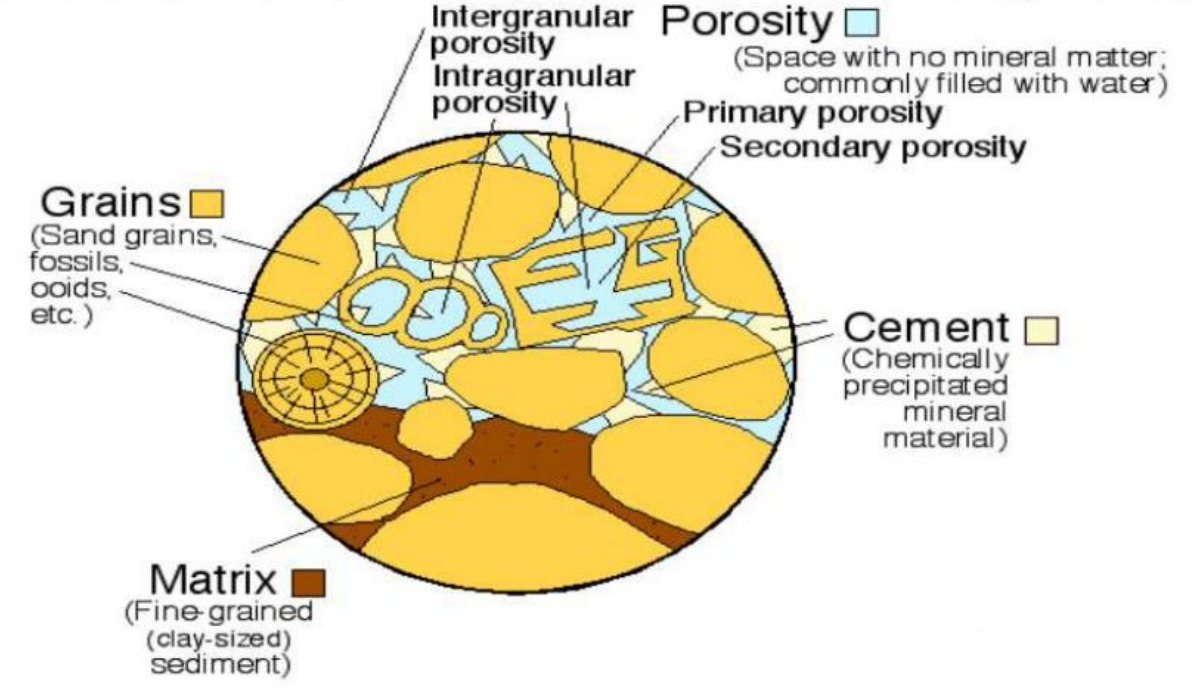
\includegraphics[width=0.9\linewidth]{img/components.jpeg}
    \caption{Four Fundamental components of sedimentary rocks}
\end{figure}

\subsubsection*{Porosity classifications}
\begin{enumerate}
    \item \textbf{Primary Porosity}:
    Primary porosity refers to the porosity that develops during the formation of the sedimentary rock itself. It is a result of depositional processes and the initial arrangement of grains or particles. Primary porosity can be further divided into three types:
    \begin{enumerate}
        \item Intergranular Porosity: This type of porosity occurs between individual grains or particles in the rock. It is common in sedimentary rocks composed of well-sorted, rounded grains, such as sandstones. The size, shape, and packing arrangement of the grains determine the degree of intergranular porosity.
        \item Intragranular Porosity: In certain cases, primary porosity can occur within individual grains. This usually happens when the grains themselves have pore spaces or contain dissolved minerals that later dissolve, leaving behind pore spaces. Intragranular porosity is commonly observed in certain limestone and chalk formations.
        \item Framework Porosity: Framework porosity refers to the pore space within the framework of the rock itself. It occurs in rocks composed of framework-forming minerals, such as some volcanic rocks or certain siliceous sandstones. The arrangement and connectivity of mineral grains determine the framework porosity.
    \end{enumerate}
    
    \item \textbf{Secondary Porosity}:
    Secondary porosity develops after the initial formation of the rock due to subsequent geological processes. It is typically associated with fluid flow and can significantly enhance the overall porosity of the rock. Some common mechanisms of secondary porosity formation include:
    \begin{enumerate}
        \item Fracturing: Tectonic forces or stress can cause rocks to fracture, creating new pore spaces. These fractures can act as conduits for fluid flow and significantly increase the permeability and porosity of the rock.
        \item Dissolution: Certain minerals, such as calcite in limestone or evaporite deposits, can dissolve over time when exposed to acidic fluids. This dissolution creates new pore spaces and enlarges existing ones, leading to increased porosity.
        \item Leaching: Leaching involves the removal of certain minerals or components from the rock by circulating fluids. This process can create pore spaces and increase the overall porosity.
    \end{enumerate}
\end{enumerate}

\subsubsection*{Factors affecting Porosity}
\begin{enumerate}
    \item Primary Porosity depends on mainly:
    \begin{itemize}
        \item Particle sphericity and angularity
        \item Sorting (variable grain sizes)
        \item Packing
    \end{itemize}

    \item Secondary Porosity depends on mainly:
    \begin{itemize}
        \item Cementing materials
        \item Overburden stress (compaction)
        \item Vugs, dissolution, and fractures
    \end{itemize}
    
\end{enumerate}

\subsection*{Idealized Packing Model}

\subsubsection*{Parallel Cylindrical Pore} 
\begin{multicols}{2}
    \begin{align*}
        \Phi &= \frac{V_p}{V_b} \\ 
        &= \frac{\pi r^2 \times n \times m }{2rn \times 2rm} \\
        &= \frac{\pi}{4} \\
        &= 78.5\%  
    \end{align*}
    here, r: Pipe radius \\
    m, n: number of cylinder contained in the bulk volume\\
    Vp: Pore volume \\
    Vb: Bulk volume
\end{multicols}

\subsubsection*{Regular Cubic Packed Sphere} 
\begin{multicols}{2}
    \begin{align*}
        \Phi &= \frac{V_p}{V_b} = \frac{V_b-V_m}{V_b} \\ 
        &= 1- \frac{\pi}{6} \\
        &= 47.6\%  
    \end{align*}
    here,$V_p$: Pore volume \\
    $V_b$: Bulk volume = $(2r)^3 = 8r^3$\\
    $V_m$ : Matrix volume = $8\times \frac{1}{8} \times \left(\frac{4}{3} \pi r^3 \right) $
\end{multicols}

\subsubsection*{Regular Orthorhombic Packed Sphere} 
\begin{multicols}{2}
    \begin{align*}
        \Phi &= \frac{V_p}{V_b} = \frac{V_b-V_m}{V_b} \\ 
        &= 1- \frac{V_m}{V_b} \\
        &= 1- \frac{4\pi r^3}{12 \sqrt{3} r^3} \\
        &= 39.5\%  
    \end{align*}
    here,$V_p$: Pore volume \\
    $V_b$: Bulk volume = $2r \times 2r \times h = 2r \times 2r \times (2r \sin 60)\\  
    \hspace{1cm} = 4 \sqrt{3}r^3$\\
    $V_m$ : Matrix volume = $8\times \frac{1}{8} \times \left(\frac{4}{3} \pi r^3 \right) $
\end{multicols}

\subsubsection*{Regular Rhombohedral Packed Sphere} 
\begin{multicols}{2}
    \begin{align*}
        \Phi &= \frac{V_p}{V_b} = \frac{V_b-V_m}{V_b} \\ 
        &= 1- \frac{V_m}{V_b} \\
        &= 1- \frac{4\pi r^3}{12 \sqrt{2} r^3} \\
        &= 26.0\%  
    \end{align*}
    here,$V_p$: Pore volume \\
    $V_b$: Bulk volume = $2r \times 2r \times h = 2r \times 2r \times (2r \sin 45)\\  
    \hspace{1cm} = 4 \sqrt{2}r^3$\\
    $V_m$ : Matrix volume = $8\times \frac{1}{8} \times \left(\frac{4}{3} \pi r^3 \right) $
\end{multicols}

\begin{figure}[h]
	\centering
  
	\subfigure[Parallel Cylindrical Pore]{
	  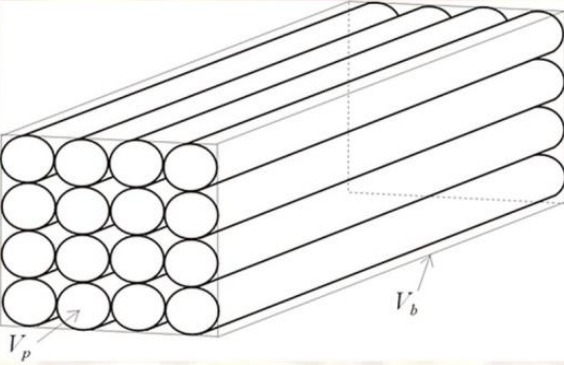
\includegraphics[width=0.45\linewidth]{img/parallel_cylindrical_pore.jpeg}
	  \label{fig:ID}
	}
	\hfill
	\subfigure[Regular Cubic Packed]{
	  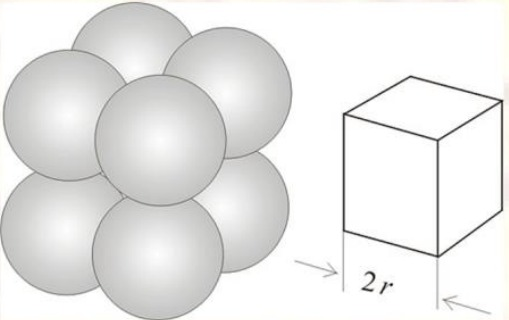
\includegraphics[width=0.45\linewidth]{img/regular_cubic_packed.jpeg}
	  \label{fig:const_vol}
	}
	
	\subfigure[Regular Orthorhombic Packed]{
	  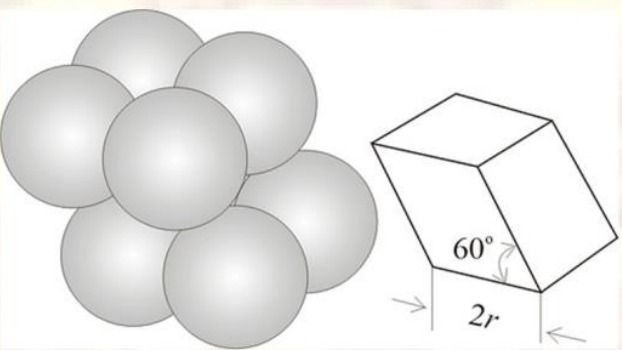
\includegraphics[width=0.45\linewidth]{img/regular_orthorhombic_packed.jpeg}
	  \label{fig:const_pressure}
	}
	\hfill
	\subfigure[Regular Rhombohedral Packed]{
	  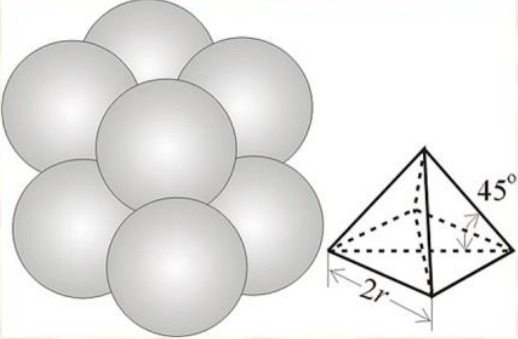
\includegraphics[width=0.45\linewidth]{img/regular_rhombohedral_packed.jpeg}
	  \label{fig:limited_const_vol_pre}
	}

    \caption{Idealized Packed Model}
	\label{fig:combustion_cycle}
  \end{figure}

  \subsection*{Factors affecting Porosity}
  \begin{enumerate}
    \item Packing Density: The arrangement and packing of sediment grains affect the amount of pore space available. Higher packing density leads to lower porosity, while looser packing allows for greater porosity.
    \item Grain Size: The size of sediment grains influences porosity. Finer-grained sediments generally have higher porosity compared to coarser-grained sediments due to the smaller size of individual grains and increased intergranular space.
    \item Sorting: Sorting refers to the uniformity of grain sizes within a sediment. Well-sorted sediments have higher porosity since there is less interference between grains, allowing for better packing and more pore space.
    \item Post Burial Change in Porosity: Burial and diagenetic processes can alter the porosity of sedimentary rocks. Factors like compaction, cementation, and dissolution can lead to changes in porosity over time.
    \item Compaction: Burial and the weight of overlying sediments cause compaction, reducing pore space and porosity. The degree of compaction depends on factors such as sediment type, burial depth, and time.
    \item Cementation: Cementation occurs when minerals precipitate in the pore spaces, binding sediment grains together. Cementation reduces porosity by filling the pore spaces with solid material.
    \item Clay Formation: Clay minerals can form during diagenesis and contribute to porosity reduction. Clay particles are very small and have a high surface area, which can lead to pore clogging and decreased overall porosity.
    \item Fracturing: Fractures, faults, and other brittle deformation features can enhance porosity in rocks. These fractures create pathways for fluid flow and can significantly increase the effective porosity of a reservoir rock.
  \end{enumerate}
  
  \subsubsection*{Some important points}
  \begin{itemize}
    \item Porosity of most reservoirs ranges from 5-30\% and the most 
    common is 10-20\%
    \item Carbonate reservoir has slightly less porosity than sandstone 
    reservoir but permeability is higher than sandstone
    \item A reservoir with less than 5\% porosity is considered less 
    commercial. Rough Field appraisal is as follows:
    \begin{itemize}
        \item 0-5\%: Negligible
        \item 5-10\%: Poor
        \item 10-15\%: Fair
        \item 15-20\%: Good
        \item 20-25\%: Very Good
    \end{itemize}
  \end{itemize}

    \section{Lecture 5: permeability \& Darcy's Equations}
    \hfill Date: 21/06/2023 

    \subsection*{permeability}
    Permeability is basically a property of the medium and is a measure of the capacity of the medium to transmit fluids.

    \subsubsection*{Permeability Theory}
    Let, Q = volumetric flow rate \\
    A = Cross sectional Area \\ 
    L = Length of porous medium \\ 
    $h_1, h_2$ = Hydraulic Head at inlet \& Outlet \\ 
    $$Q \propto \frac{h_1 - h_2}{L} $$
    $$Q \propto A $$
    \begin{figure*}[h]
        \begin{center}
            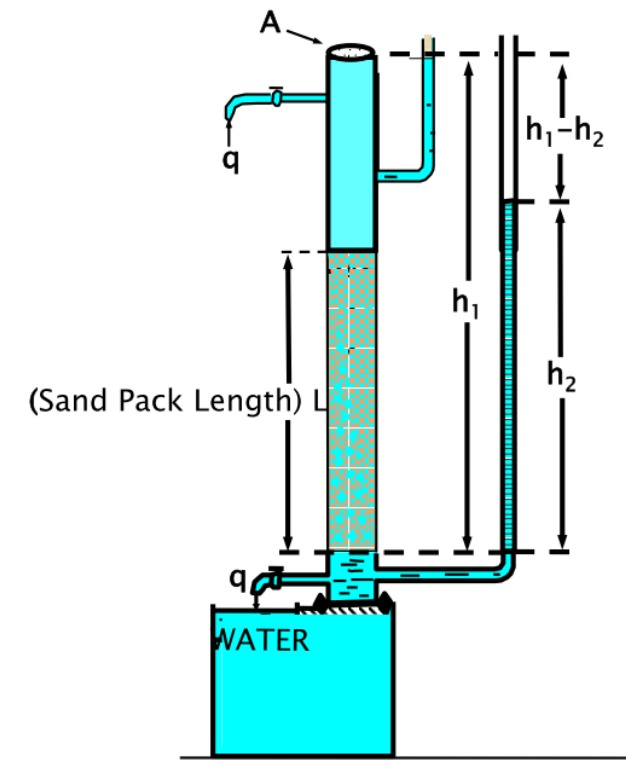
\includegraphics[width=0.5\linewidth]{img/darcy_apparatus.jpeg}
            \caption{Darcy apparatus for determining permeability}
        \end{center}
    \end{figure*}

    \subsubsection*{Extension of Darcy's Equation}
    In Darcy's equation, he didn't considered the viscous effect. But, other researchers showed that, volumetric flow rate in inversely proportional to viscosity. Also, he restricted to a medium with 100\% saturation. 

    \subsubsection*{Assumptions for Extension of Darcy's Equation}
    \begin{enumerate}
        \item Steady state flow, under laminar
        regime i.e. $Q_{in} = Q_{out}$
        \item Viscous flow - rate of flow directly proportional to pressure gradient
        \item The flowing fluid is incompressible.
        \item Porous media 100\% saturated with flowing fluid
        \item Fluid and porous media not reacting       
    \end{enumerate}

    The equation is represented by - 
    $$Q = - \frac{k}{\mu} A \dfrac{dp}{dL}$$
    here, $\mu$ = Viscosity of given fluid \\
    k = permeability of porous medium \\ 

    \begin{figure}[h]
        \centering
      
        \subfigure[Extension of Darcy's equation]{
          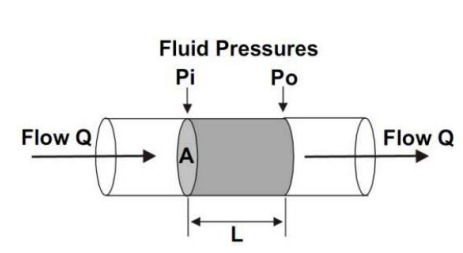
\includegraphics[width=0.45\linewidth]{img/darcy_eqn.jpeg}
          \label{fig:darcy}
        }
        \hfill
        \subfigure[Unit of Darcy]{
          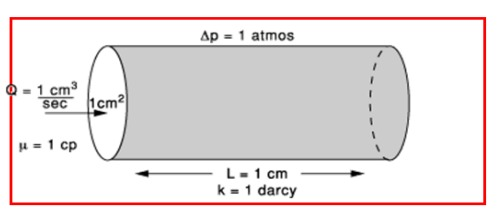
\includegraphics[width=0.45\linewidth]{img/unit_darcy.jpeg}
          \label{fig:unit_darcy}
        }
    
        \caption{Extension of Darcy's Equation}
        \label{fig:Extension of Darcy's Equation}
      \end{figure}

      \subsubsection*{Unit of permeability}
      \textbf{A porous medium is said to have a permeability value of one Darcy when a single phase fluid having a viscosity of one centipoise (cP) completely saturates the porous medium and flows through it at a rate of 1 $cm^3/sec$ under a viscous flow regime and a pressure gradient of 1 $atm/cm$ through a cross sectional area of 1 $cm^2$.}

    \begin{align*}
        k &= \frac{- Q \mu}{A \frac{dp}{dL}} \\
        1 Darcy &= \frac{cm^3/sec \times cP}{cm^2 \times atm/cm} \\ 
        1 D &= 9.869 \times 10^{-9} \, cm^2 \\
        &= 9.869 \times 10^{-13} \, m^2 \\
        &= 1.062 \times 10^{-11} \, ft^2 
    \end{align*}

    \begin{multicols}{2}
        Generally Permeability is termed as: 
        \begin{itemize}
            \item Poor : $k < 1$
            \item Fair : $1< k < 10$
            \item Moderate : $10< k < 50$
            \item Good : $50< k < 250$
            \item Very Good : $ k > 250$
        \end{itemize}
    
        \subsubsection*{Factors affecting the permeability}
        \begin{enumerate}
            \item Diameter of the pathways 
            \item The tortuosity of the pathways 
        \end{enumerate}
    
        \subsubsection*{Sediment controls of permeability}
        \begin{enumerate}
            \item Packing density  
            \item Porosity 
            \item Grain size 
            \item Sorting 
            \item Post burial process 
        \end{enumerate}

        \vspace*{0.5cm}
    \end{multicols}

    \subsection*{Darcy's Equation of Linear Flow}
    \begin{align*}
        Q &= - \frac{k}{\mu} A \frac{dP}{dL} \\
        \frac{Q}{A} dx &= -\frac{k}{\mu} dP \\
        \frac{Q}{A} \int_{0}^{L} \, dx &= -\frac{k}{\mu} \int_{P_1}^{P_2} \, dP \\
        \frac{Q}{A} (L-0) &= - \frac{k}{\mu} (P_2 - P_1) \\
        \therefore Q &= \frac{kA}{\mu} \frac{(P_1-P_2)}{L}
    \end{align*}

    \subsubsection*{Darcy’s equation for linear Parallel flow}
    $$h = h_1 + h_2 + h_3 = \sum h_i$$
    $$p_1 - p_2 = \Delta p_1 = \Delta p_2 = \Delta p_3$$
    $$Q = Q_1 + Q_2 + Q_3 = \sum Q_i$$

    Total flow in terms of average permeability:
    $$Q = \frac{\overline{k}Wh}{\mu L} \Delta P $$

    now,
    \begin{align*}
        Q &= Q_1 + Q_2 + Q_3 \\
        \frac{\overline{k}Wh}{\mu L} \Delta P  &= \frac{k_1Wh_1}{\mu L} \Delta P_1 + \frac{k_2Wh_2}{\mu L} \Delta P_2 + \frac{k_3Wh_3}{\mu L} \Delta P_3 \\
        \frac{\overline{k}Wh}{\mu L} \Delta P  &= \frac{k_1Wh_1}{\mu L} \Delta P + \frac{k_2Wh_2}{\mu L} \Delta P + \frac{k_3Wh_3}{\mu L} \Delta P \\ 
        \overline{k} &= \frac{\sum k_ih_i}{\sum h_i}
    \end{align*}

    \begin{figure}[h]
        \centering
      
        \subfigure[Linear Parallel Flow]{
          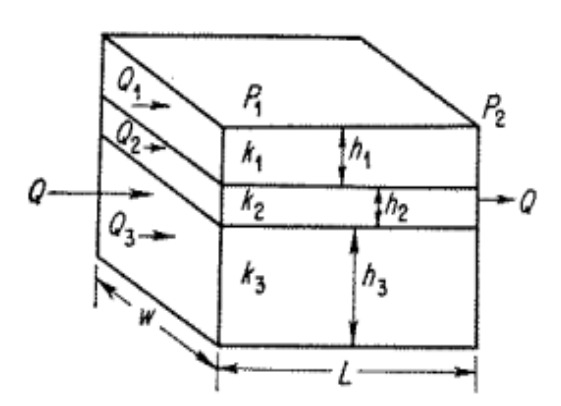
\includegraphics[width=0.45\linewidth]{img/linear_parallel.jpeg}
          \label{fig:linear_parallel}
        }
        \hfill
        \subfigure[Linear Series Flow]{
          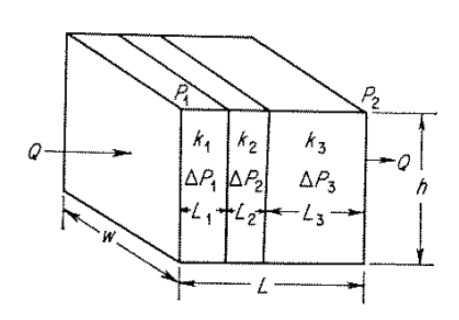
\includegraphics[width=0.45\linewidth]{img/linear_series.jpeg}
          \label{fig:linear_series}
        }
    
        \caption{Linear flow}
        \label{fig:Linear flow}
      \end{figure}

    \subsubsection*{Darcy’s equation for linear Series flow }
    $$L = L_1 + L_2 + L_3 = \sum L_i$$
    $$p_1 - p_2 = \Delta p_1 + \Delta p_2 + \Delta p_3$$
    $$Q = Q_1 = Q_2 = Q_3 $$

    Total pressure drop in terms of average permeability:
    $$P_1 - P_2 = \frac{Q \mu L}{\overline{k}W h}$$
    now, 
    \begin{align*}
        p_1 - p_2 &= \Delta p_1 + \Delta p_2 + \Delta p_3 \\ 
        \frac{Q \mu L}{\overline{k}W h} &= \frac{Q \mu L_1}{k_1W h} + \frac{Q \mu L_2}{k_2W h} + \frac{Q \mu L_3}{k_3W h} \\
        \frac{L}{\overline{k}} &= \frac{L_1}{k_1} + \frac{L_2}{k_2} + \frac{L_3}{k_3} \\
        \overline{k} &= \frac{\sum L_i}{\sum \dfrac{L_i}{k_i}}
    \end{align*}

    \subsection*{Darcy's Equation of Radial Flow}

    \begin{align*}
        Q &= \frac{kA}{\mu} \frac{dP}{dL} \\
        Q &= \frac{k (2 \pi r h)}{\mu} \frac{dP}{dL} \\
        Q \frac{dr}{2\pi r h} &= \frac{k}{\mu} dP \\
        \frac{Q}{2\pi h} \int_{r_w}^{r_e} \frac{dr}{r} &= \frac{k}{\mu} \int_{P_{wf}}^{P_e} dP \\
        \frac{Q}{2 \pi h} \ln \frac{r_e}{r_{wf}} &= \frac{k}{\mu} \left(P_e-P_{wf}\right) \\
        Q &= \frac{2\pi h k \left(P_e - P_{wf}\right)}{\mu \left(\ln \left(\frac{r_e}{r_{wf}}\right)\right)}
    \end{align*}

    \subsubsection*{Darcy’s equation for Radial Parallel Flow}
    $$h = h_1 + h_2 + h_3 = \sum h_i$$
    $$p_e - p_w = \Delta p_1 = \Delta p_2 = \Delta p_3$$
    $$Q = Q_1 + Q_2 + Q_3 = \sum Q_i$$

    Total flow in terms of average permeability:
    $$Q = \frac{2\pi h k }{\mu \ln \left(\frac{r_e}{r_{wf}}\right)} \Delta P $$

    now,
    \begin{align*}
        Q &= Q_1 + Q_2 + Q_3 \\
        \frac{2\pi h \overline{k} \left(P_e - P_{wf}\right)}{\mu \left(\ln \left(\frac{r_e}{r_{wf}}\right)\right)}  &= \frac{2\pi h_1 k_1 \left(P_e - P_{wf}\right)}{\mu \left(\ln \left(\frac{r_e}{r_{wf}}\right)\right)} + \frac{2\pi h_2 k_2 \left(P_e - P_{wf}\right)}{\mu \left(\ln \left(\frac{r_e}{r_{wf}}\right)\right)} + \frac{2\pi h_3 k_3 \left(P_e - P_{wf}\right)}{\mu \left(\ln \left(\frac{r_e}{r_{wf}}\right)\right)} \\ 
        \overline{k} &= \frac{\sum h_ik_i}{h} =\frac{\sum h_ik_i}{\sum h_i}
    \end{align*}

    \begin{figure}[h]
        \centering
      
        \subfigure[Radial Parallel Flow]{
          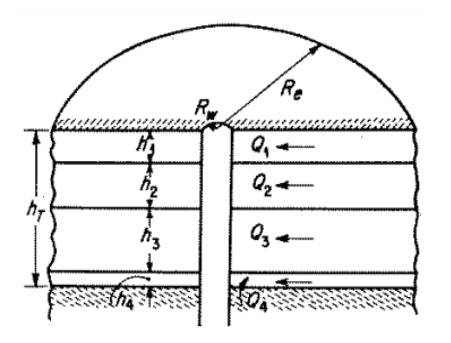
\includegraphics[width=0.49\linewidth]{img/radial_parallel.jpeg}
          \label{fig:radial_parallel}
        }
        \hfill
        \subfigure[Radial Series Flow]{
          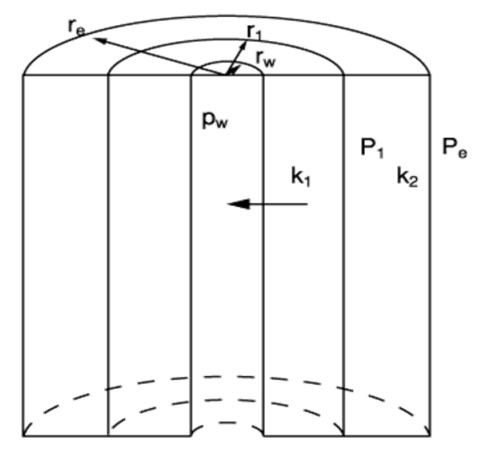
\includegraphics[width=0.40\linewidth]{img/radial_series.jpeg}
          \label{fig:radial_series}
        }
    
        \caption{Radial Flow}
        \label{fig:Radial flow}
      \end{figure}

    \subsubsection*{Darcy’s equation for Radial Series flow }
    $$p_e - p_w = \Delta p_1 + \Delta p_2 + \Delta p_3$$
    $$Q = Q_1 = Q_2 = Q_3 $$

now,
\begin{align*}
    P_e - P_w &= (P_e-P_1)+(P_1-P_w) \\ 
    \frac{Q_T \mu \ln \frac{r_e}{r_w}}{2\pi \overline{k}_{avg} h} &= \frac{Q_1 \mu \ln \frac{r_1}{r_w}}{2\pi k_1 h} + \frac{Q_2 \mu \ln \frac{r_e}{r_1}}{2\pi k_2 h} \\
    \overline{k}_{avg} &= \sum_{i=1}^{n} \frac{\ln \left(\frac{r_i}{r_{i-1}}\right)}{k_i}
\end{align*}

\section{Lecture 06: Wettability} 
\hfill Date: 11/07/2023

\textbf{Follow the slide of Wettability!!}
\vspace*{1cm}

\end{document}